% !TEX TS-program = pdflatex
% !TEX encoding = UTF-8 Unicode

% This is a simple template for a LaTeX document using the "article" class.
% See "book", "report", "letter" for other types of document.

\documentclass[10pt]{article} % use larger type; default would be 10pt

\usepackage[utf8]{inputenc} % set input encoding (not needed with XeLaTeX)
\usepackage[QX]{fontenc}
\usepackage{lmodern}

%%% Examples of Article customizations
% These packages are optional, depending whether you want the features they provide.
% See the LaTeX Companion or other references for full information.

%%% PAGE DIMENSIONS
\usepackage{geometry} % to change the page dimensions
\geometry{a4paper} % or letterpaper (US) or a5paper or....
 \geometry{margin=0.5in} % for example, change the margins to 2 inches all round
% \geometry{landscape} % set up the page for landscape
%   read geometry.pdf for detailed page layout information

\usepackage{graphicx} % support the \includegraphics command and options
\usepackage{listings}
% \usepackage[parfill]{parskip} % Activate to begin paragraphs with an empty line rather than an indent

%%% PACKAGES
\usepackage{booktabs} % for much better looking tables
\usepackage{array} % for better arrays (eg matrices) in maths
\usepackage{paralist} % very flexible & customisable lists (eg. enumerate/itemize, etc.)
\usepackage{verbatim} % adds environment for commenting out blocks of text & for better verbatim
\usepackage{subfig} % make it possible to include more than one captioned figure/table in a single float
% These packages are all incorporated in the memoir class to one degree or another...

%%% HEADERS & FOOTERS
\usepackage{fancyhdr} % This should be set AFTER setting up the page geometry
\pagestyle{fancy} % options: empty , plain , fancy
\renewcommand{\headrulewidth}{0pt} % customise the layout...
\lhead{}\chead{}\rhead{}
\lfoot{}\cfoot{\thepage}\rfoot{}

%%% SECTION TITLE APPEARANCE
\usepackage{sectsty}
\allsectionsfont{\sffamily\mdseries\upshape} % (See the fntguide.pdf for font help)
% (This matches ConTeXt defaults)

%%% ToC (table of contents) APPEARANCE
\usepackage[nottoc,notlof,notlot]{tocbibind} % Put the bibliography in the ToC
\usepackage[titles,subfigure]{tocloft} % Alter the style of the Table of Contents
\renewcommand{\cftsecfont}{\rmfamily\mdseries\upshape}
\renewcommand{\cftsecpagefont}{\rmfamily\mdseries\upshape} % No bold!

%%% END Article customizations

%%% The "real" document content comes below...


\title{Metody numeryczne zadanie nr 3}
\author{Mateusz Miotk \\  Sylwia Kaczmarczyk \\ Michał Kulesz}
%\date{} % Activate to display a given date or no date (if empty),
         % otherwise the current date is printed 

\begin{document}
\maketitle

\section{Treść zadania}
$\textbf{Zadanie 3.1} $ Zagadnienie różniczkowe: $y'=2y^2 -2x(x^3 - 1) , y(1)=1 $\\
rozwiązać na przedziale $[1,3]$ metodą Eulera oraz zmodyfikowaną metodą Eulera zwaną metodą punktu środkowego.\\
Wyniki porównać z rozwiązaniem dokładnym $y(x) = x^2$.

\section{Podstawy teoretyczne}
\subsection{Metoda Eulera}
Niech będzie dane równanie różniczkowe zwyczajne $y' = f(x,y(x))$ z warunkiem początkowym $y(x_0) = y_0$\\
Metoda Eulera polega na zastąpieniu krzywej całkowej $y = y(x)$ przechodzącej przez punkt $M_0(x_0,y_0)$, odpowiadający 
warunkom początkowym, łamaną $M_0,M_1,M_2,..,$ o wierzchołkach $M_i(x_i,y_i) , i=0,1,2,...,$ składającą się z odcinków prostych.\\
Wykorzystywane jest tutaj dane rownanie rekurencyjne: \\
%$\left\{\begin{array}  y_1 = y(x_0)+hf(x_0,y(x_0))\\y_{i+1} = y_i + hf(x_i,y_i)\end{array}}$
$$
 \left\{ \begin{array}{ll}
 y_0 = y(x_0)\\
 y_1 = y_0+hf(x_0,y_0)\\
y_{i+1} = y_i + hf(x_i,y_i)\\
\end{array} \right.
$$
\\gdzie h jest krokiem na osi x.\\
\subsection{Zmodyfikowana metoda Eulera}
Idea jest podobna ale wykorzystywany jest inny wzór rekurencyjny: \\
$$
 \left\{ \begin{array}{ll}
 y_0 = y(x_0)\\
 y_1 = y_0+hf(x_0 + \frac{h}{2},y_0 + f(x_0,y_0)\cdot\frac{h}{2})\\
 y_{i+1} = y_i+hf(x_i + \frac{h}{2},y_i + f(x_i,y_i)\cdot\frac{h}{2})\\
\end{array} \right.
$$
\section{Algorytm realizujący zadanie}
\subsection{Algorytm}
1.Program będzie wymagał od użytkownika "dopóki mu się nie znudzi" parametru h gdzie $h \in [0,1]$\\
2.Następnie dla danego parametru h w przedziale $[1,3]$ będzie liczone rozwiązanie metodą Eulera oraz Zmodyfikowaną metodą Eulera według wzorów podanych powyżej. \\
3.Zostanie wypisana tabela ilustrująca poszczególne kroki metody a na końcu zostaną wypisane minimalne i maksymalne błędy osiągane przez obydwie metody.\\
\subsection{Przykładowe rozwiązanie}
Dla h = 0.5 rozwiązanie wynosi:\\
$\begin{tabular}{c|c|c|c|c|c}
$x_0$ & $Y_{euler}$ & $Y_{mid}$ &Dokładne&$Błąd_{euler}$&$Błąd_{midpoint}$\\ 
1.500000    &    2.000000       & 2.058594           & 2.250000       & 0.250000       & 0.191406\\ \hline
2.000000        & 2.437500       & 0.171691           & 4.000000       & 1.562500       & 3.828309\\ \hline
2.500000        & -5.621094      & 23.217517         & 6.250000       & 11.871094     & 16.967517\\ \hline
3.000000        & -10.586899    & 75298.618184   & 9.000000       & 19.586899     & 75289.618184\\ 
\end{tabular}
$\\\\
Dla h = 0.25 rozwiązanie wynosi:\\
$\begin{tabular}{c|c|c|c|c|c}
$x_0$ & $Y_{euler}$ & $Y_{mid}$ &Dokładne&$Błąd_{euler}$&$Błąd_{midpoint}$\\ 
1.250000        &1.500000       &1.542847       &1.562500       &0.062500       &0.019653\\ \hline
1.500000        &2.029297       &2.136079       &2.250000       &0.220703       &0.113921\\ \hline
1.750000        &2.307070       &2.309015       &3.062500       &0.755430       &0.753485\\ \hline
2.000000        &1.153902       &-1.428743      &4.000000       &2.846098       &5.428743\\ \hline
2.250000        &-5.180353      &-0.800476      &5.062500       &10.242853      &5.862976\\ \hline
2.500000        &-3.451778      &5.506390       &6.250000       &9.701778       &0.743610\\ \hline
2.750000        &-15.775641     &-9.136616      &7.562500       &23.338141      &16.699116\\ \hline
3.000000        &81.439086      &-40.096835     &9.000000       &72.439086      &49.096835\\
\end{tabular}$



\section{Opis programu}
\subsection{Opis struktur danych oraz funkcji w programie}
Program składa się w głównej mierze z liczb zmiennoprzecinkowych:\\
$max_blad_Euler$ maksymalny błąd osiągany metodą Eulera\\
$min_blad_Euler$ minimalny błąd osiągany metodą Eulera\\
$max_blad_Mid$ maksymalny błąd osiągany metodą Zmodyfikowaną metodą Eulera\\
$min_blad_Mid$ minimalny błąd osiągany metodą Zmodyfikowaną metodą Eulera\\
\Najwazniejsze funkcje uzyte w programie to:\\
1. Wczytywanie zmiennej h\\
2. Sprawdzanie, czy $h \in [0,1]$\\
3. Liczenie rozwiązanie metodą Eulera oraz Zmodyfikowaną metodą Eulera\\
4. Wypisanie tabeli poszczególnych kroków\\
5. Wypisanie największy oraz najmniejszy błąd osiągane przez poszczególne metody\\
\subsection{Opis wejścia-wyjścia}
Program na początku chce otrzymać zmienną h, która spełnia warunki opisane w punkcie 3.\\
Program sprawdzi, czy podana wartość spełnia warunek. Jeżeli nie, to wyświetli odpowiedni komunikat.\\
Następnie program wykona obliczenia metodami Eulera oraz Zmodyfikowaną metodą Eulera i będzie wyświetlał na ekranie poszczególne kroki.\\
Potem program wyświetli największy oraz najmniejszy błąd dla poszczególnych metod.\\
Po tym wszystkim użytkownik może podać kolejną wartość h, dopóki mu się nie znudzi.\\
\subsection{Treść programu}
\begin{lstlisting}
#include <stdio.h>
#include <stdlib.h>
#include <math.h>
double abs_double(double x){
	if(x <0)
	return -1.0*x;
	else
	return x;
}
double f_dokladne(double x){
	return x*x;
}
double f(double x,double y){
	return 2*y*y - 2*x*x*x*x+2*x;
}
void Euler(double h){
double x_0,y_0;
double x_temp,y_temp,blad;
double y_0_mid,y_temp_mid,blad_mid;
double max_blad_Euler,max_blad_Mid;
double min_blad_Euler,min_blad_Mid;
max_blad_Euler = max_blad_Mid =0.0;
min_blad_Euler = min_blad_Mid = INFINITY; 
x_0 = 1;
y_0 = 1;
y_0_mid=1;
printf("X_0    \t\t|Y       \t|Y_mid  \t|Dokladne\t|Blad_Euler\t|Blad_MidPoint\n");
printf("--------------------------------------------------------------------------------------------\n");
while(1){
	x_temp = x_0 + h;
	if(x_temp <= 3){
	y_temp = y_0+h*f(x_0,y_0);
	y_temp_mid = y_0_mid+h*f(x_0+(h/2),y_0_mid+(f(x_0,y_0_mid)*h/2));
	x_0 = x_temp;
	y_0 = y_temp;
	y_0_mid=y_temp_mid;
	blad=abs_double(f_dokladne(x_0) - y_0);
	blad_mid=abs_double(f_dokladne(x_0)-y_0_mid);
	if(max_blad_Euler < blad){
	max_blad_Euler = blad;
	}
	if(max_blad_Mid < blad_mid){
	max_blad_Mid = blad_mid;
	}
	if(min_blad_Euler > blad){
	min_blad_Euler=blad;
	}
	if(min_blad_Mid > blad_mid){
		min_blad_Mid = blad_mid;
	}
printf("%lf\t|%lf \t|%lf\t|%lf\t|%lf\t|%lf\n",x_0,y_0,y_0_mid,f_dokladne(x_0),blad,blad_mid);
	}
else{
printf("Maksymalny blad w metodzie Eulera wynosi: %lf\n",max_blad_Euler);
printf("Maksymalny blad w metodzie Mid_Point wynosi: %lf\n",max_blad_Mid);
printf("Minimalny blad w metodzie Eulera wynosi: %lf\n",min_blad_Euler);
printf("Minimalny blad w metodzie Mid_point wynosi: %lf\n",min_blad_Mid);
break;
}
		
}
}
int poprawnosc_h(double h){
	if(h <= 0 || h>=1)
	return -1;
	else
	return 1;
}

void pobranie_danych(){
	double h;
	while(1){
		printf("Podaj h: Ctrl+c konczy dzialanie programu\n");
		scanf("%lf",&h);
		if(poprawnosc_h(h)==1){
		Euler(h);
		}
		else
		printf("Wartosc h nie jest w przedziale (0,1)");
	}
}

int main(){
	pobranie_danych();
	return EXIT_SUCCESS;
}
\end{lstlisting}
\subsection{Zrzuty wybranego programu}
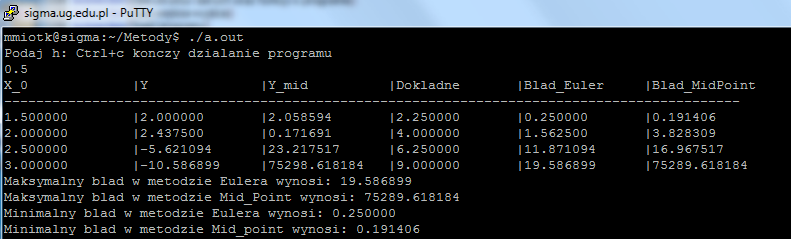
\includegraphics{metody1.png}\\\\\\\\
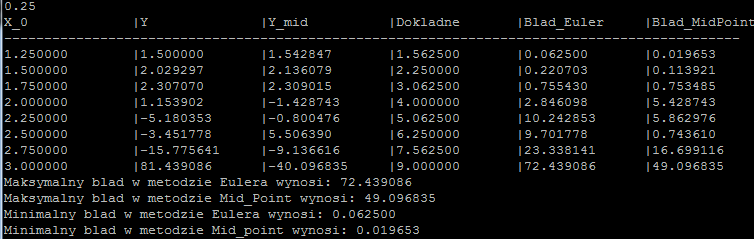
\includegraphics{metody2.png}
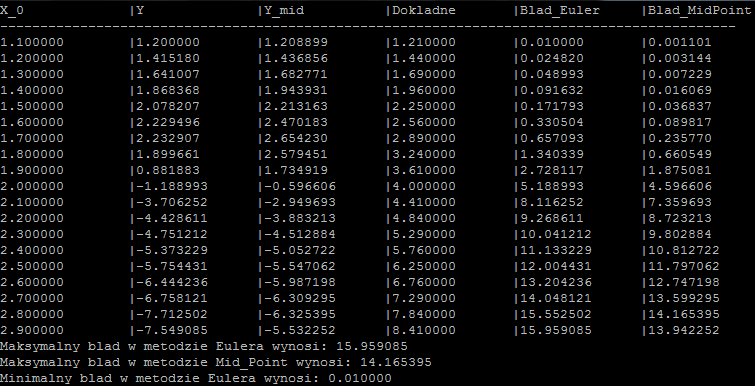
\includegraphics{metody3.png}

\end{document}
